% 学位论文 : 第二章 实验技术及设备简介
% 
% 更新记录:
%   {$LastChangedBy$}
%   {$LastChangedRevision$}
%   {$LastChangedDate$}

\chapter{实验技术及设备简介}
\section{生长设备}

现代半导体材料科学重点研究基于各种半导体微结构的光电信息功能材料,与之相对应,半导体材料主流制备技术也由拉单晶、液相外延等体材料、厚膜材料生长技术转向气相外延、真空淀积等超薄层、低维量子结构材料生长技术。现有的外延生长技术手段主要有液相外延、气相外延、分子束外延、金属有机物化学气相沉积,表\ref{tab:growth_methods}将这几种技术做了详尽的比较。

\begin{table*}[htbp] 
	\centering
	\caption{\label{tab:growth_methods}外延生长技术手段}  
	\begin{tabular}{m{.15\textwidth}<{\centering}m{.1\textwidth}<{\centering}m{.25\textwidth}m{.2\textwidth}m{.2\textwidth}}  
		\toprule
			外延生长方法 & 发明时间 & 特点 & 优势 & 劣势 \\
		\midrule 
			液相外延(Liquid Phase Epitaxy) & 1963 & 从过饱和溶液中析出固相物质并沉积在衬底上 & 简单;纯度高 & 扩展性和均匀性差 \\
			气相外延(Vapor Phase Epitaxy) & 1958 & 采用金属卤化物输运 & 简单;纯度高 & 不能外延所有合金;没有突变界面;外延层较厚 \\
			分子束外延(Molecular Beam Epitaxy) & 1958-1967 & 在超高真空条件下沉积外延层 & 过程简单;外延薄膜纯度高;生长速率缓慢 & 很难生长As/P合金;不利于批量生长 \\
			金属有机物化学气相沉积(MOCVD) & 1968 & 用金属有机物作为源 & 几乎可生长任意化合物;反应室简单;可批量生长 & 反应物价格高;参数控制严格;源毒性大 \\
		\bottomrule
	\end{tabular}
\end{table*}


分子束外延(MBE)技术和金属有机物化学气相沉积(MOCVD)技术是其中两项最具有代表性的超薄层、低维量子结构材料生长技术,可以用来制备最小厚度达到亚纳米量级的、高质量的半导体超薄层、二维量子阱、超晶格材料。采用应变自组装技术,还可以利用MBE和MOCVD技术获得高质量的一维量子线材料和零维量子点材料。

在本研究中我们采用MOCVD技术生长所需要的外延材料。MOCVD技术始于1968年Manasevi的早期工作,他在蓝宝石上进行了多种III-V族半导体材料的异质外延生长\cite{epitaxial-growth.1}\cite{epitaxial-growth.2}\cite{epitaxial-growth.3}。随着能带工程、量子效应等半导体物理的进展以及对器件速度、频率、功率等性能的不断追求,使得MOCVD取得了令人瞩目的进展。今天MOCVD已经成为研究与制备化合物半导体异质结、超晶格材料、量子点等低维结构以及生产化合物半导体光电子、微电子器件的重要方法。MOCVD方法的优点是具有生长多种高纯化合物半导体材料的灵活性,能够生长大面积、均匀的外延层,并可精确控制极薄层材料的厚度、组分、掺杂和界面。因此,MOCVD技术不但用于化合物半导体材料和器件的研发,还适用于生产。MOCVD方法的主要缺点是需要使用大量的有毒气体(诸如$AsH_3$、$PH_3$、$H_2Se$等)和在空气中自然的金属有机化合物,以及与空气能形成易爆混合物的氢气。
下面我们主要介绍一下MOCVD的生长机理。

{\hei 金属有机化合物化学气相沉积}
金属有机化合物化学气相沉积(MOCVD),又称金属有机化合物气相外延(MOVPE)、有机金属化合物气相外延(OMVPE),他是利用金属有机化合物进行金属输运的一种气相外延生长技术\cite{Wang2005}。

MOCVD技术现已获得广泛应用,成为制备化合物半导体异质结、低维结构材料,以及生产化合物半导体光电子、微电子器件的重要方法。用MOCVD技术生产半导体激光器、发光管、太阳能电池和高频、高速电子器件等都已形成产业。

MOCVD通常采用III族、II族元素的金属有机化含物和V族、VI族的气态氮化物等作为III-V族或II-VI族晶体生长的反应源。在MOCVD外延生长中,载气($H_2$或$N_2$)把金属有机化合物和非金属氢化物的蒸汽输运到高温反应的区域,即携带到反应室中加热的衬底上方,随着温度的升高在气相和气相-固相界面发生一系列的化学和物理变化,最终在衬底表面生成外延层。

以三甲基镓(TMGa)和砷化氢($AsH_3$)生长GaAs为例,化学反应可简化表示为:

\begin{equation}
	\label{eq:GaAsGrowth}
	(CH_3)_3Ga + AsH_3 \rightarrow GaAs + CH_4
\end{equation}


其中GaAs沉积到晶体表面,CH4挥发到气相中,离开反应室。
图\ref{fig:mocvd}是GaAs外延的示意图。

\begin{figure}[h]
	\centering
	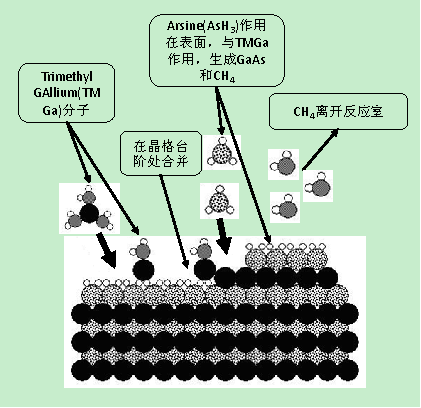
\includegraphics[width=0.8\textwidth]{ch02_MOCVD.pdf}
	\caption{MOCVD}
	\label{fig:mocvd}
\end{figure}


整个MOCVD外延生长过程,如上图所示,具体可分为如下步骤:
\begin{enumerate}[(1)]
	\setlength{\itemsep}{-3pt}
	\item III族源(MO源)和V族源(如HydrideGas)注入到反应室中;
	\item 反应源混合均匀后,被载气(一般是H2)输运到沉积区域;
	\item 在沉积区域,高温导致反应源的分解及其它气相反应,生成了薄膜生长所需的源(Film Precursors)及一定的副产物;
	\item Film Precursors通过扩散输运到晶体生长表面;
	\item Film Precursors被表面吸附;
	\item Film Precursors扩散到生长位置;
	\item 通过表面反应,薄膜生长所需的原子并入到外延薄膜中,而表面反应的副产物则从晶体表面脱附;
	\item 表面反应的副产物输运回远离沉积区域的主气流中,进而通过尾气管道排出反应室。
\end{enumerate}

在实验过程中我们所采用的是从英国Thomas Swan Scientific Equipment Limited(TSSEL是德国Aixtron集团的子公司)公司购置的3X2”CCS InP型LP-MOCVD设备。该MOCVD设备可以分为5个主要的子系统:源输送系统(GasDeliverySystem)、反应室与加热系统、低压系统(Low Pressure Exhaust System)、尾气处理系统(Scrubbering System)及安全与控制单元(Safety\&ControlUnit)。


\section{表征设备}

半导体材料的应用主要取决于材料的光学和电学性能,而后者又完全取决于材料的电子能带结构、化学成分、晶体结构以及可能存在的各种缺陷等。为了掌握材料的光电性能极其影响因素,人们开发出了各种各样的材料表征技术。这些技术提供了关于半导体的物理性能、结构性能和器件性能的互补信息。在本研究中我们主要关注半导体材料的表面形貌和结构特性,因此我们主要采用的半导体材料表征技术包括(如图\ref{fig:view}):原子力显微镜(AFM)、X射线衍射仪(XRD)、透射电子显微镜(TEM)、扫描电子显微镜(SEM)和腐蚀坑设备等。

\begin{figure}[!htb]
	\centering
	\subfigure[原子力显微镜(AFM)] {
		\label{fig:AFM}
		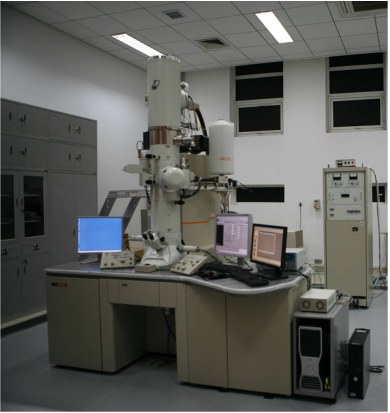
\includegraphics[width=1.5in]{ch02_TEM.pdf}
	} 
	\subfigure[X射线衍射仪(XRD)] {
		\label{fig:XRD}
		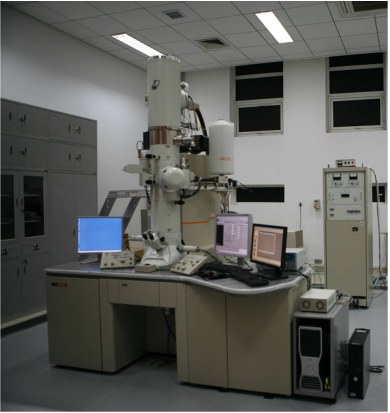
\includegraphics[width=1.5in]{ch02_TEM.pdf}
	} 
	\subfigure[透射电子显微镜(TEM)] {
		\label{fig:TEM}
		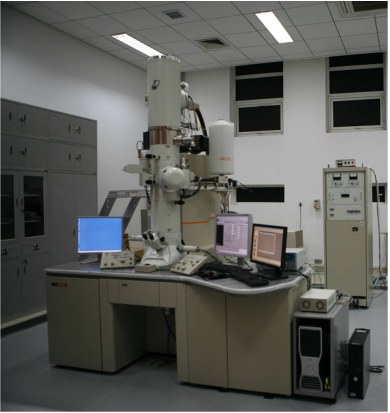
\includegraphics[width=1.5in]{ch02_TEM.pdf}
	} 
	\subfigure[扫描电子显微镜(SEM)] {
		\label{fig:SEM}
		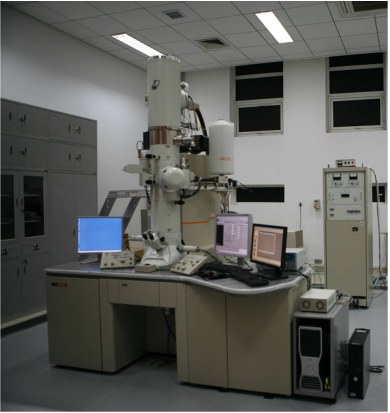
\includegraphics[width=1.5in]{ch02_TEM.pdf}
	}
	\subfigure[腐蚀坑设备] {
		\label{fig:XXX}
		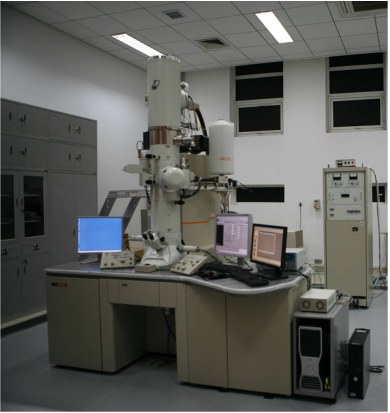
\includegraphics[width=1.5in]{ch02_TEM.pdf}
	}  
	\caption{表征设备}
	\label{fig:view}
\end{figure}

{\hei 原子力显微镜}
原子力显微镜是一种超高分辨率的扫描探针显微镜,它所具有的纳米级分辨率超过了光学衍射极限的1000倍。1986年binning, Calvin Quate和Gerber在扫描隧道显微镜的基础上发明了第一台原子力显微镜。AFM成像是通过探针在样品表面扫描移动来实现的,通过探针受力的变化来获取表面形貌的信息,可以在不同的模式下运行,包括接触模式、非接触模式和轻敲模式。
接触模式:
接触模式是指在AFM扫描的整个过程中,探针的针尖切入样品表面,两者始终紧密接触,探针与样品表面的作用力是排斥力,并保持很定,该模式对探针和样品表面都有损伤。
非接触模式:
在非接触模式下,探针与样品表面并不接触,而是以高于两者的共振频率的频率振动,通过控制探针与样品表面的平均距离,维持不变的振动频率和振幅,测量每个数据点上两者之间的距离即可构建出样品表面形貌,该模式中两者之间的作用力是范德华力,并且不会对探针和样品表面造成损伤。
轻敲模式
轻敲模式是指探针周期性地短暂德敲击样品表面,其中探针是以两者的共振频率振荡,通过控制探针与样品表面的距离,保持振动振幅,成像两者之间的相互作用力得到样品表面形貌图像,改模式不会对探针和样品表面造成损伤。
我们所使用的AFM设备是

{\hei X-射线衍射仪}
X射线技术是半导体薄膜材料结构性质研究中最常用的一种手段,利用X射线技术可以精确地获得半导体外延层的成分、厚度、应变等结构信息。XRD是利用X射线衍射原理研究物质内部结构的大型分析仪器,由于其测试方法简单且精度高,常用于晶体质量的测试。
1912年,劳厄预想:由于X射线的波长和晶体原子之间距离相近,所以可以把晶体作为X射线的衍射光栅,当X射线照到晶体上时,原子发生散射,并产生衍射波,这些波互相干涉,产生衍射。衍射波相互叠加,使得射线在某些方向上加强,而在其他方向上减弱,分析衍射结果,就能够得到晶体结构,这一预想后被实验证实。1913年,Bragg父子在这基础上成功测得了NaCl、KCl等晶体结构,并提出了布拉尔方程:2dsinθ=nλ。
XRD便是利用这一原理测定物质的晶体结构,它主要由高稳定度X射线源、样品及样品位置取向的调整机构系统、射线检测器和衍射图的处理分析系统组成。
在本研究中,我们使用XRD来表征晶体质量,所使用的XRD设备是


\begin {figure}
	\begin{minipage}[t]{0.45\linewidth}
		\centering
		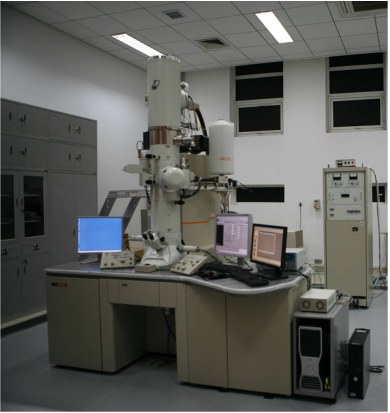
\includegraphics[width=1.2in]{ch02_TEM.pdf}
		\caption{透射电子显微镜(TEM)}
		\label{fig:TEM}
	\end{minipage}%
	\begin{minipage}[t]{0.45\linewidth}
		\centering
		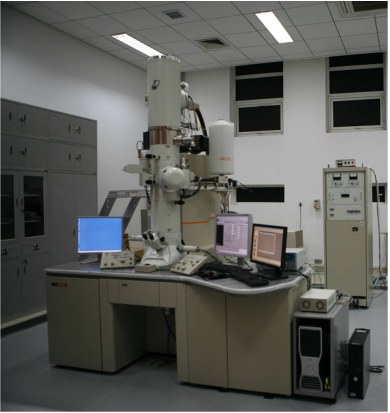
\includegraphics[width=1.2in]{ch02_TEM.pdf}
		\caption{扫描电子显微镜(SEM)}
		\label{fig:SEM}
	\end{minipage}
\end{figure}


{\hei 透射电子显微镜}
透射电子显微镜(Transmission electron microscope,缩写TEM),是利用电子的波动性原理直接观察固体材料的原子结构和各种缺陷的仪器,通过把经过加速和聚集的电子束投射到非常薄的样品上,经过与原子碰撞,电子改变方向产生了立体角散射。由于散射角的大小和样品的厚度、密度相关,从而形成了明暗不同的影像。1931年,克诺尔和鲁斯卡研制出了第一台透射电子显微镜。
与光学显微镜相比,透射电子显微镜的分辨率要高很多,能够达到0.1~0.2nm,可以放大几万~百万倍。所以,利用透射电子显微镜可以观察到样品的精细结构,甚至是一列原子的结构。
在本研究中,我们采用TEM来观察外延片的厚度和位错形成,我们使用的是北京大学物理学院电子显微镜专业实验室的JEM-2100F场发射透射电子显微镜,设备如Figure 1所示。该设备的最小分辨率可达到0.2nm。

{\hei 扫描电子显微镜}
扫描电子显微镜(scanning electron microscope,简称SEM)是利用二次电子信号成像来观察样品的表面形态。利用高能的入射电子轰击物质表面,被激发区域将产生二次电子、俄歇电子、X射线、电磁辐射等,同时也会产生电子-空穴对、声子等,根据电子与物质所产生的相互作用,便能够获取被测样品的形貌、组成、晶体结构等信息。扫描电子显微镜就是利用电子束扫描样品,激发出二次电子,由于二次电子的数量与电子束入射角即样品表面结构有关,通过探测器收集二次电子,将其转变为光信号,便能扫描出样品表面结构的图像。它主要由三大部分组成:真空系统、电子束系统及成像系统。
我们使用SEM主要观察外延片厚度和腐蚀坑形貌,我们选用的是清华大学电子工程系的HITACHI S-5500场发射扫描电子显微镜,其分辨率可达到0.4nm。

{\hei 腐蚀坑设备}
在GaAs/Si异变外延材料中,由于GaAs与Si之间的晶格失配与热失配,导致产生了大量位错,这些位错极大的限制了材料的应用,因此对于材料位错特性的表征显得尤为重要,在本研究中,我们除采用XRD、TEM之外表征材料质量之外,还采用了腐蚀坑密度来表征位错密度。
通过腐蚀坑表征位错密度有以下几种方法:熔融KOH法\cite{Grabmaier1969},阳极腐蚀法\cite{Cao1980},AB腐蚀法\cite{Abrahams1965}等,我们采用的是已经形成国家标准方法的KOH腐蚀法。GaAs/Si外延片经熔融KOH腐蚀后,晶体表面的位错露头处,腐蚀速度较快,而没有位错的表面腐蚀速度较慢,这就形成了带棱角的具有特定形状的腐蚀坑。而GaAs单晶的腐蚀条件比较宽松,当熔化的KOH呈现澄清状态时,选择适当的腐蚀时间,就能够得到清晰的腐蚀坑形貌。通过扫描电子显微镜观察这些腐蚀坑的形貌,这些腐蚀坑的密度便在一定程度上表征了外延片的位错密度。在腐蚀坑测试过程中,由于两个或更多的位错线会交错到一起形成一个大坑,所以并不是每条位错线都能够形成腐蚀坑,这就导致了腐蚀坑密度要小于外延片实际的位错密度\cite{}。


% 本章参考文献
\ifx\usechapbib\empty
\bibliographystyle{buptthesis}
\bibliography{bare_thesis}
\fi


%%% Local Variables: 
%%% mode: latex
%%% TeX-master: "bare_thesis"
%%% End: 
